
\section{Experiments and Discussion}
\label{sec:experiments}
In this section, we experiment on binary classification for both artificial dataset (i.e., Moon) for demonstration and real-world datasets (i.e., Breast Cancer, Credit Card Fraud). Samples in artificial Moon have two dimensions while samples in Breast Cancer and Credit Card Fraud are both 30-dimension numerical data. Compare to the original Breast Cancer dataset size (569 samples), the other original Credit Card dataset contains a much larger amount of data, 284,907 samples. 
The implementation steps to balance datasets are following Algorithm \ref{alg:SIMPOR}. To evaluate our proposed balancing technique, we compare the classification performance to different widely-used techniques. More specifically, We compare \Methodname{} to SMOTE \cite{chawla_smote:_2002}, Borderline-SMOTE \cite{bordersmote},  ADASYN \cite{ADASYN}, Random Oversampling, and Raw data which does not apply any balancing technique. To evaluate classifications performance for skewed datasets, we measure some powerful and widely-used metrics such as Recall, Precision, F1-score, Area Under The Curve (AUC). %and Receiver Operating Characteristic Curve (ROC).    


\begin{table}[]
	\centering
	\caption{Classification models' setting for each dataset.}
	%\rule{\linewidth}{3cm}
	\label{tab:model_setting}
	\resizebox{\columnwidth}{!}{%
		\begin{tabular}{p{6.145em}lccccc}
			\multicolumn{1}{l}{Model Setting} &     &     Moon       &     & \multicolumn{1}{l}{Breast Cancer} &     & \multicolumn{1}{l}{Credit Card} \\
			\cmidrule{1-1}\cmidrule{3-3}\cmidrule{5-5}\cmidrule{7-7}
			\multicolumn{1}{l}{Hidden Layers} &     & 3   &     & 3   &     & 3 \\  
			Neurons/Layer &     & 100 &     & 50  &     & 200 \\
			\multicolumn{1}{l}{Hidden Activation} &     & ReLu &     & ReLu &     & ReLu \\
			\multicolumn{1}{l}{Output Activation} &     & Softmax &     & Softmax &     & Softmax \\
			Epochs &     & 200 &     & 150 &     & 200 \\
			\multicolumn{1}{l}{Batch size} &     & 32  &     & 32  &     & 64 \\
			Optimizer &     & Adam &     & Adam &     & Adam \\
			Learning Rate &     & 0.01 &     & 0.01 &     & 0.01 \\
			\bottomrule
		\end{tabular}%
	}
	
\end{table}%

\subsection{Sharing Settings}
This subsection describes settings sharing for all datasets. In order to find the informative subset, we leverage entropy-based active learning as mentioned in Section \ref{sec:EAL}. Classifier for active learning is a fully connected neural network model containing 3 hidden layers with \textit{relu} activation functions and 100 neurons each layer. The output layer uses softmax activation function. The models are trained in a maximum of 300 epochs with the early stop option when the loss does not change after updating weights. 

In addition, we randomly split the data into two parts, 80\% for training and 20\% for testing. Reported testing results for each dataset are the averages of 5 experimental trials. For \Methodname{} to find optima of the function in Equation \ref{prob:optimazation}, we use a gradient ascent rate of 0.00001 and the maximum iteration of 300. The architecture detail of the evaluation model for each dataset is described in Table \ref{tab:model_setting}.



\subsection{\Methodname{} on artificial Moon dataset}

\begin{figure*}[tp]
	\centering
	%[trim=left bottom right top, clip]
	\begin{subfigure}[]{0.3\linewidth}	
		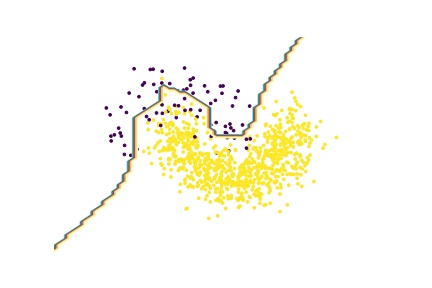
\includegraphics[width=\linewidth]{Figures/moon/RawData}
		\caption{Raw Data. \\F1 = 0.852}
		\label{fig:raw_moon}
	\end{subfigure}
	\hspace{0.1em}% 
	\begin{subfigure}[]{0.3\linewidth}
		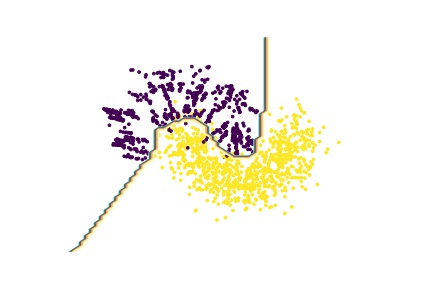
\includegraphics[width=\linewidth]{Figures/moon/SIMPOR_global1}
		\caption{\Methodname{}.\\F1 = 0.917}
		\label{fig:simpor_moon}
	\end{subfigure}
	\hspace{0.1em}% 
	\begin{subfigure}[]{0.3\linewidth}
		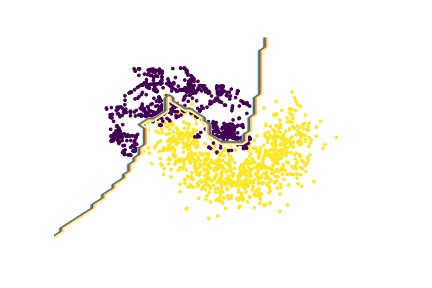
\includegraphics[width=\linewidth]{Figures/moon/SMOTE}
		\caption{SMOTE. \\F1 = 0.862}
		\label{fig:smote_moon}
	\end{subfigure}
	\\
	\begin{subfigure}[]{0.3\linewidth}
		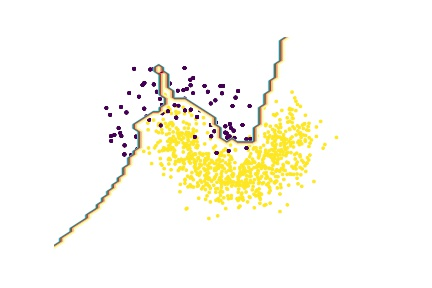
\includegraphics[width=\linewidth]{Figures/moon/OverSampling}
		\caption{ Random Over Sampling.\\  \centering{F1 = 0.834 }}
		\label{fig:oversampling_moon}
	\end{subfigure}
	\hspace{0.1em}% 
	\begin{subfigure}[]{0.3\linewidth}
		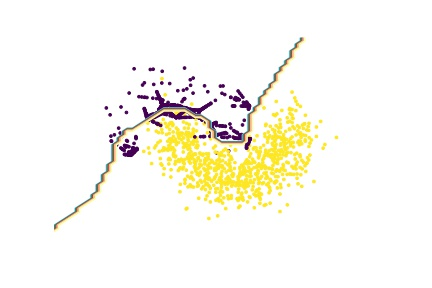
\includegraphics[width=\linewidth]{Figures/moon/BorderlineSMOTE}
		\caption{BorderlineSMOTE.\\F1 = 0.827}
		\label{fig:border_smote_moon}
	\end{subfigure}
	\hspace{0.1em}% 
	\begin{subfigure}[]{0.3\linewidth}
		\includegraphics[width=\linewidth]{Figures/moon/AdaSYN}
		\caption{ADASYN.\\  \centering{F1 = 0.817} }
		\label{fig:adasyn_moon}
	\end{subfigure}
	
	\caption{Balanced training data plot, model's decision boundary plot and testing F1 score for Moon Dataset.}
	\label{fig:MoonResults}
\end{figure*}


We implement our technique on an artificial 2-dimension numeric dataset as a demonstration of our proposed method. Figure \ref{fig:MoonResults} captures the classification F1 results for different techniques. We also visualize model decision boundaries to provide additional information on how the classification models are affected. To classify the data, we use a fully connected neural network which is described in Table \ref{tab:model_setting}.

\subsubsection{Dataset}

We first generate a balanced dataset using python library \textit{sklearn.datasets.make\_moons} including 3000 two-dimensional samples labeled in two classes, A and B. We then create an imbalanced dataset with an Imbalance Ratio of 3:1 by randomly removing 1000 samples from class B. As a result, the training dataset becomes imbalanced as visualized in Figure \ref{fig:raw_moon}, which contains 400 samples of class B and 1200 samples of class A. The testing data contains 100 samples of class B and 300 samples of class A. 


\subsubsection{Results and Discussion}
From the results shown in Figure \ref{fig:MoonResults}, it is clear that \Methodname{} performs better than others at the F1 score of 0.9170 (Figure \ref{fig:simpor_moon}). Without any balancing techniques, it is not surprising that the classification result on the raw imbalanced data achieves the lower F1 Score, at 0.852 (Figure \ref{fig:raw_moon}). SMOTE technique does help to improve the classification F1-score to 0.862; however, it has not reached \Methodname's performance. Other techniques perform poorly in this case; they could not achieve an F1-score as high as the raw data can achieve.  

Additionally, \Methodname{}, from our observation, results in a smooth and robust model decision boundary. We can see that the Random Over Sampling which randomly duplicates minority samples might cause overfitting where samples are duplicated many times and significantly increase their weights. SMOTE does better than Random Over Sampling. However, due to the fact that SMOTE does not take the informative region into account, unbalanced data in this area lead to a severe error in decision boundary. In Figures \ref{fig:adasyn_moon} and \ref{fig:border_smote_moon}, BorderlineSMOTE and ADASYN focus on the area near the model's decision boundary, but they inherit a drawback from SMOTE; any noise or mislabeled samples can create very dense bridges crossing the expected border so that it leads to decision errors. In contrast, by generating neighbors of samples in the direction towards the minority class and balancing the informative region, \Methodname{} (Figure \ref{fig:simpor_moon}) helps the classifier to make a better decision with a solid smooth decision line. It is also worth noticing that the classifier decision boundary lines of all other techniques are rougher than that of \Methodname. This is because they randomly generate synthetic samples, and it might cause data imbalance in the informative region.

\subsection{\Methodname{} on Breast Cancer dataset}

\subsubsection{Dataset}
Breast Cancer is a real-world dataset containing information on cancer patients collected by Dua and Graff \cite{breast_cancer}. This has two classes including 357 negatives and 212 positives; each record includes 30 features extracted from a digitized image of a fine needle aspirate of a breast mass e.g., radius, area, and perimeter. Some of the records in the training dataset are randomly removed to create different imbalance ratios.  


\subsubsection{Results and Discussions}  

\begin{table*}[th!]
	\centering
	\caption{Classification results of different data balancing techniques on Breast Cancer Dataset.}
	\label{tab:breastCancerResult}
	
	\begin{tabular}{rrcrcccccc}
		\toprule
		\multicolumn{10}{c}{\textbf{     Breast Cancer}} \\
		&       &       &       &       &       &       &       &       &  \\
		\multicolumn{1}{c}{Majority:Minority} &       & Metric &       & \textbf{SIMPOR} & \textbf{SMOTE} & \textbf{Borderline} & \textbf{Over-} & \textbf{ADASYN} & \textbf{RawData} \\
		\multicolumn{1}{c}{(IR)} &       &       &       &       &       & \textbf{SMOTE} & \textbf{Sampling} &       &  \\
		\cmidrule{1-1}\cmidrule{3-3}\cmidrule{5-10}          &       & F1    &       & \textbf{0.953} & 0.931 & 0.891 & 0.935 & 0.835 & 0.944 \\
		\multicolumn{1}{c}{357:120 } &       & AUC   &       & \textbf{0.974} & \textbf{0.974} & 0.964 & \textbf{0.974} & \textbf{0.974} & 0.971 \\
		\multicolumn{1}{c}{(3:1)} &       & Precision &       & 0.970  & 0.924 & 0.868 & 0.935 & 0.790  & \textbf{0.975} \\
		&       & Recall &       & \textbf{0.938} & \textbf{0.938} & 0.922 & 0.936 & 0.928 & 0.919 \\
		\cmidrule{1-1}\cmidrule{3-3}\cmidrule{5-10}          &       & F1    &       & \textbf{0.943} & 0.903 & 0.865 & 0.939 & 0.821 & 0.879 \\
		\multicolumn{1}{c}{357:50} &       & AUC   &       & \textbf{0.968} & \textbf{0.968} & 0.967 & 0.967 & \textbf{0.968} & 0.966 \\
		\multicolumn{1}{c}{(7:1)} &       & Precision &       & \textbf{0.952} & 0.899 & 0.846 & 0.948 & 0.805 & 0.873 \\
		&       & Recall &       & \textbf{0.936} & 0.918 & 0.903 & 0.932 & 0.879 & 0.907 \\
		\bottomrule
	\end{tabular}%
	
\end{table*}%


%\begin{figure}[t!]
%	
%	\centering
	
%	%[trim=left bottom right top, clip]
%	\begin{subfigure}[]{1\linewidth}	
%		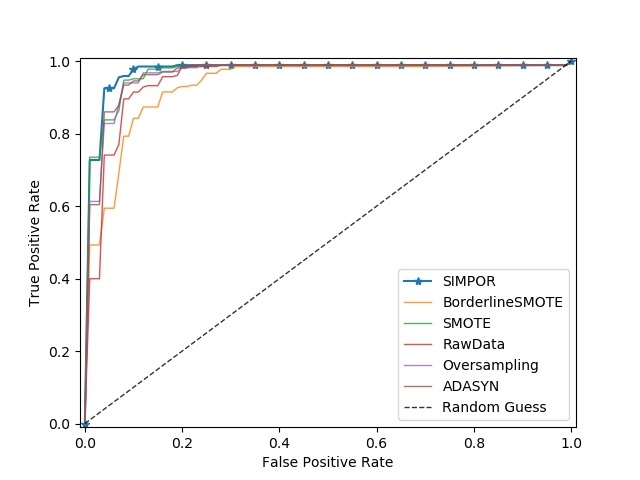
\includegraphics[width=\linewidth]{Figures/breast_cancer/3-1_ROC.jpg}
%		\caption{IR 3:1}
%		\label{fig:ROC_breastcancer_31}
%	\end{subfigure}
%	\hspace{0.1em}% 
%	\begin{subfigure}[]{1\linewidth}
%		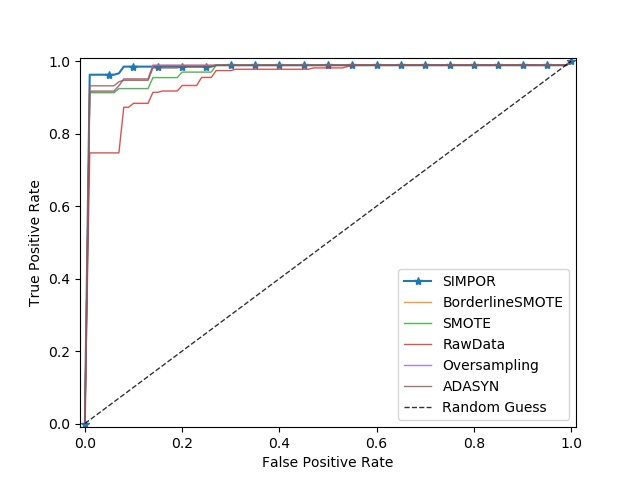
\includegraphics[width=\linewidth]{Figures/breast_cancer/7-1_ROC.jpg}
%		\caption{IR 7:1}
%		\label{fig:ROC_breastcancer_71}
%	\end{subfigure}
%	\hspace{0.1em}% 
%	
%	\caption{AUC-ROC Curve for Breast Cancer on two different Imbalance Ratios.}
%	\label{fig:ROC_breastcancer}
%\end{figure}
%





Table \ref{tab:breastCancerResult} shows the classification results of different data balancing techniques on the Breast Cancer dataset over the imbalance ratios of 3:1 and 7:1. Overall, \Methodname{} outperforms other techniques on both imbalance ratios at an F1-score of 0.947 and 0.935 for IR of 3:1 and 7:1, respectively. \Methodname{} also achieves the highest AUC results at 0.977 and 0.986 for both imbalance ratios. Both tests over the raw data (without any balancing technique) received the lowest F1-score as expected. 


%Figure \ref{fig:ROC_breastcancer} shows the receiver operating characteristic curve (ROC) which illustrates the ability of the classifiers. %As shown in the figure, \Methodname{}'s ROC curves are closest to the upper left corner. In other words, \Methodname{} reaches higher true %positive rates and lower fall positive rates.
%



\subsection{\Methodname{} on Credit Card Fraud}


\begin{figure*}[h!]
	\centering
	%[trim=left bottom right top, clip]
	\begin{subfigure}[]{0.3\linewidth}	
		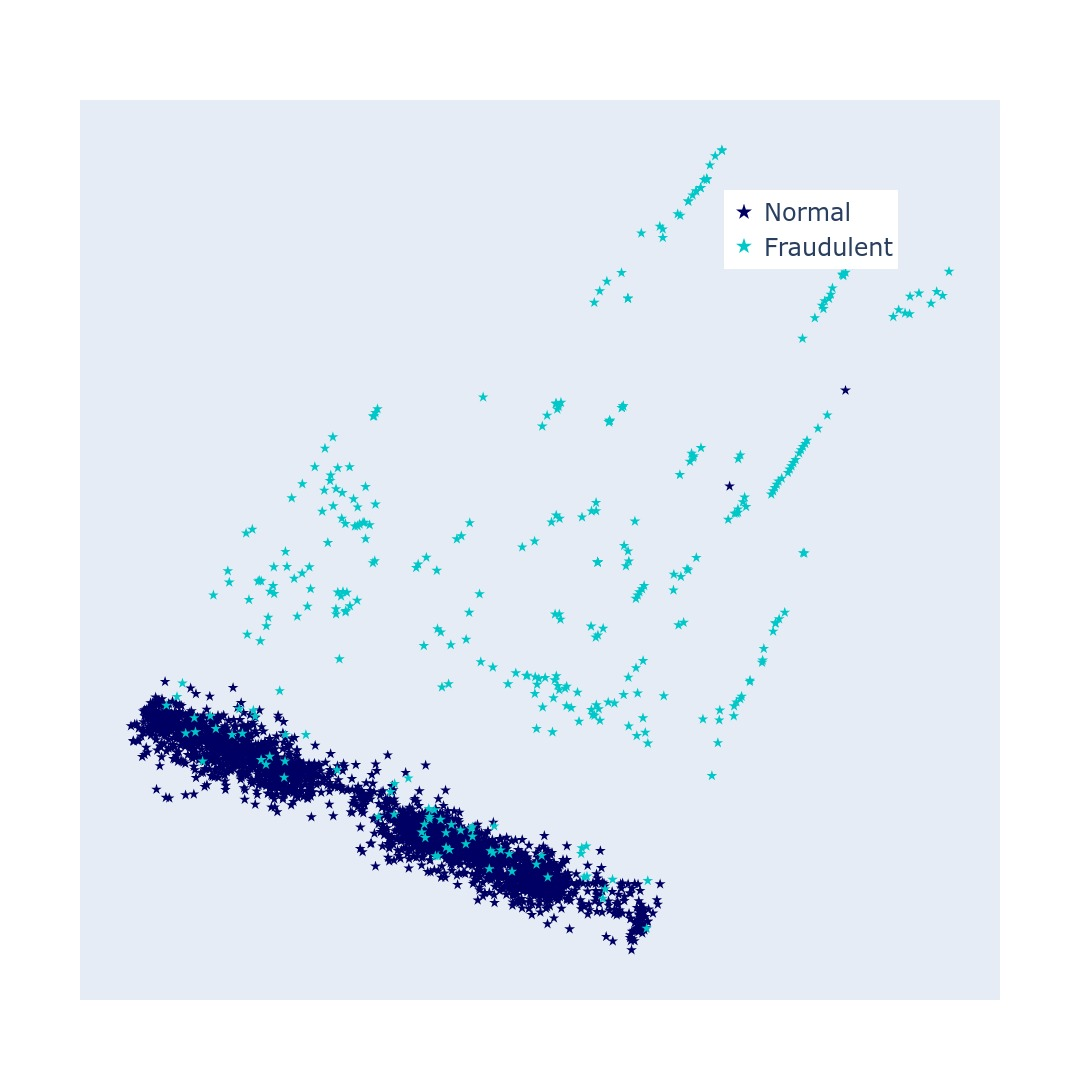
\includegraphics[width=\linewidth,trim=40 40 40 40]{Figures/creditcard/PCA/RawData-data-run-0-0}
		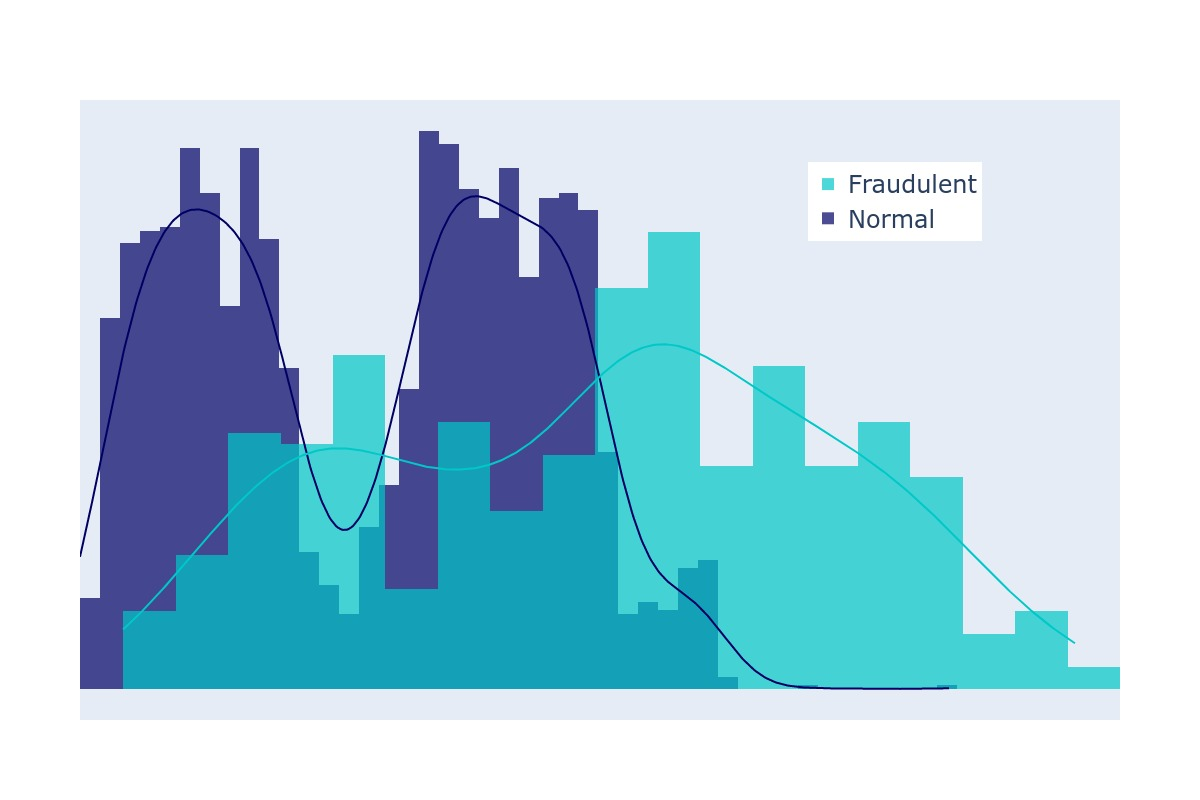
\includegraphics[width=\linewidth,trim=40 40 40 40]{Figures/creditcard/PCA/RawData-data-run-0-0_DIST}
		\begin{tabular}{c|c|c|c}
			Fraud & Normal & Inter. & HDR  \\
			\hline
			367  & 2585  & 256 & 69.75\(\%\) \\
		\end{tabular}
		\caption{Raw Data. }
		\label{fig:RawData_hist}
	\end{subfigure}
	\hspace{0.1em}%
	\begin{subfigure}[]{0.3\linewidth}	
		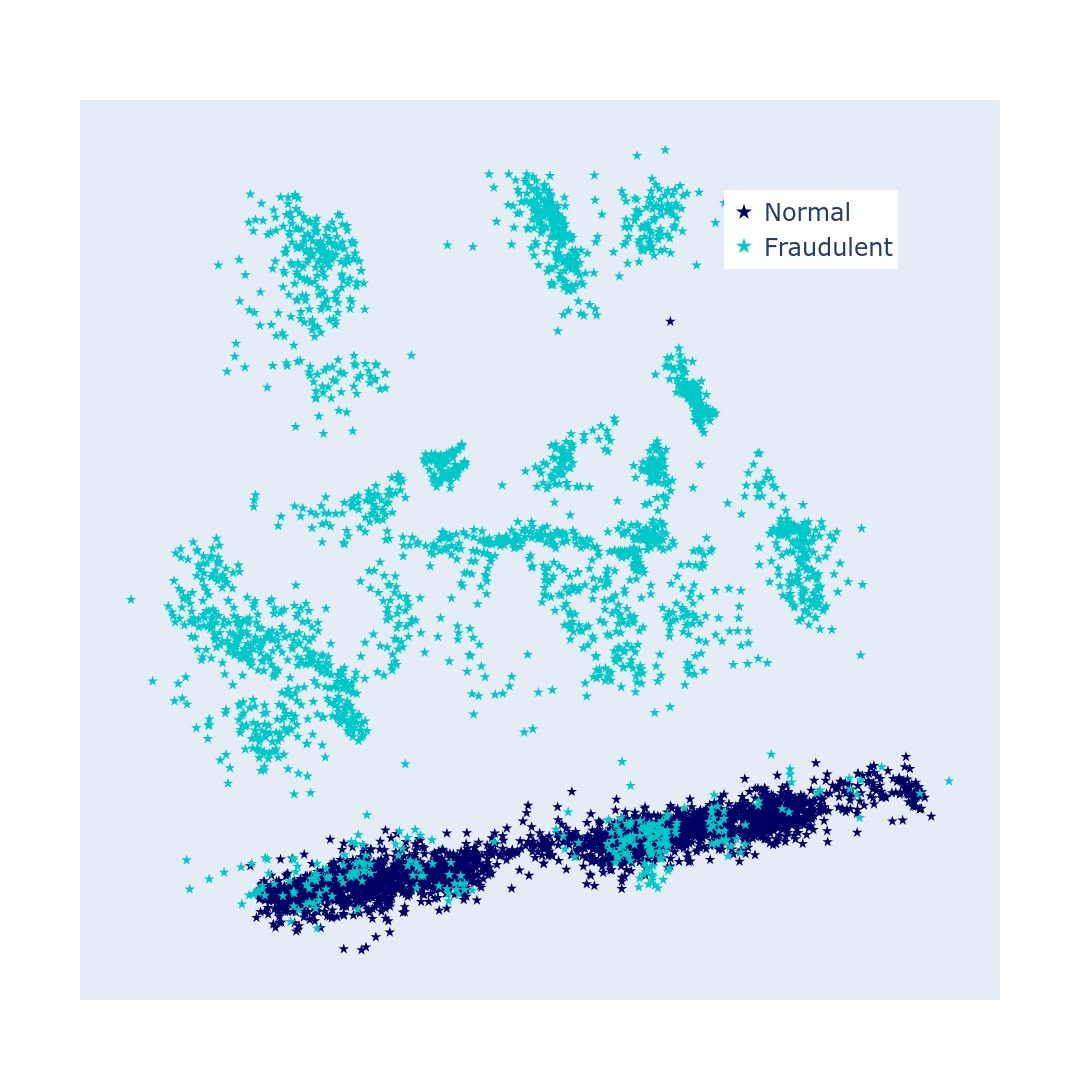
\includegraphics[width=\linewidth,trim=40 40 40 40,clip]{Figures/creditcard/PCA/SIMPOR-data-run-0-0}
		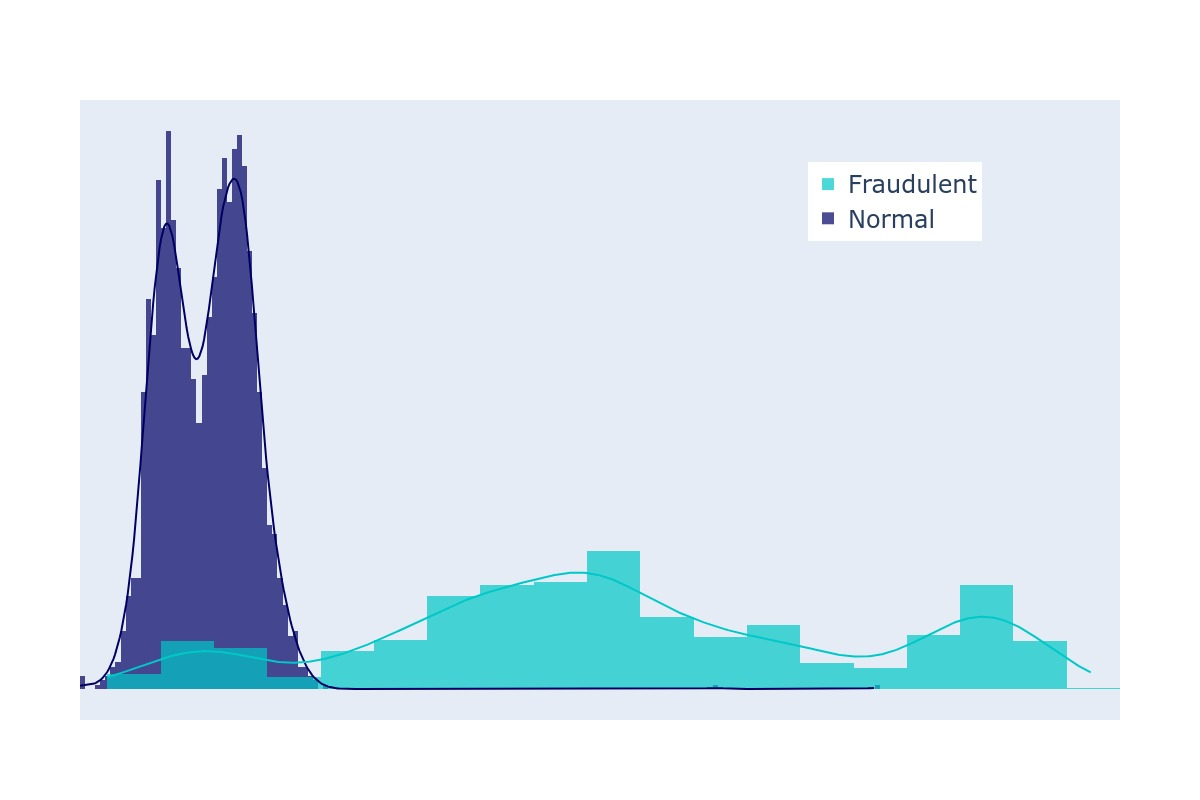
\includegraphics[width=\linewidth,trim=40 40 40 40,clip]{Figures/creditcard/PCA/SIMPOR-data-run-0-0_DIST}
		\begin{tabular}{c|c|c|c}
			Fraud & Normal & Inter. & HDR  \\
			\hline
			2585  & 2585  & 288 & \textbf{11.14\(\%\)} \\
		\end{tabular}
		\caption{Generated data by SIMPOR. }
		\label{fig:SIMPOR_hist}
	\end{subfigure}
	\hspace{0.1em}%
	\begin{subfigure}[]{0.3\linewidth}	
		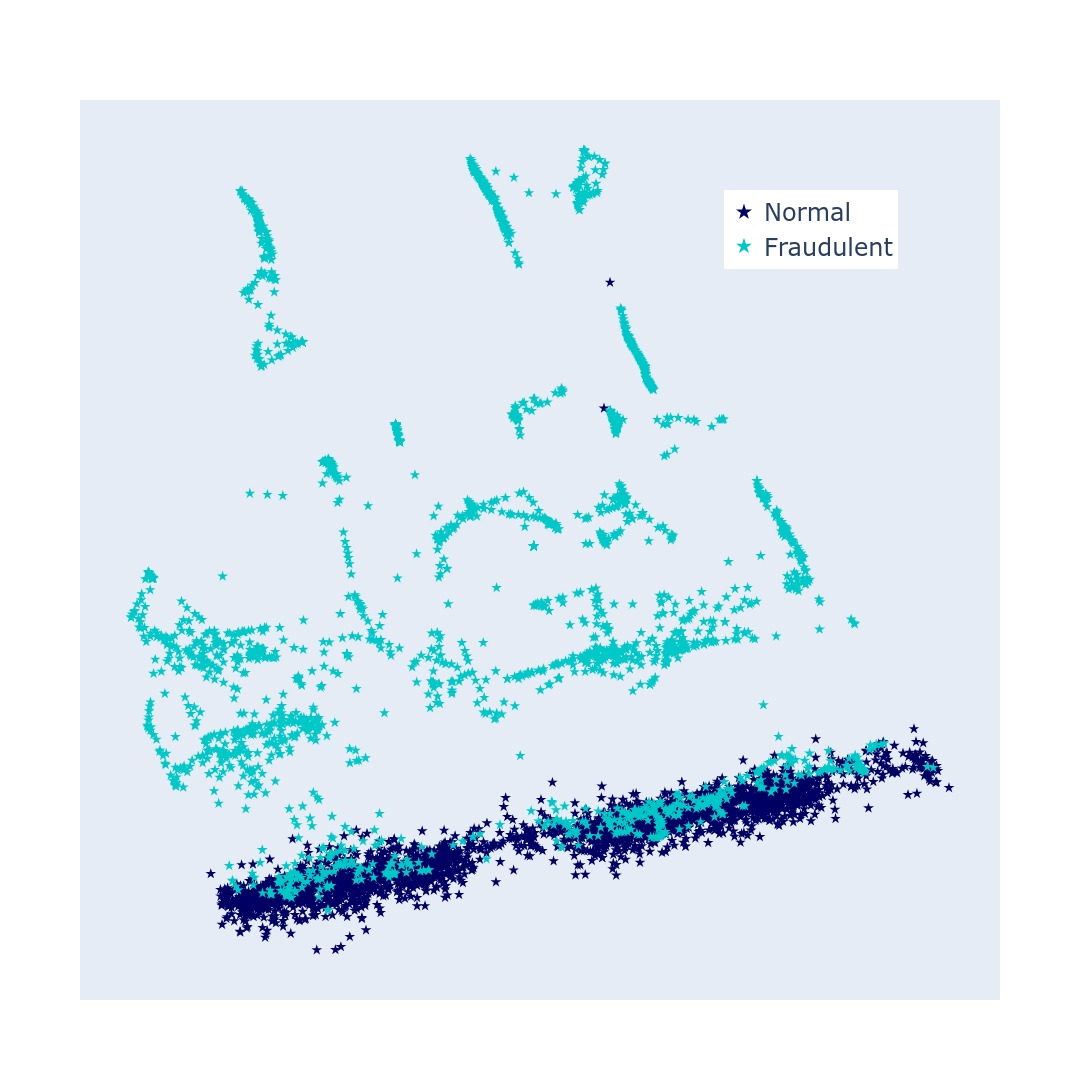
\includegraphics[width=\linewidth,trim=40 40 40 40,clip]{Figures/creditcard/PCA/SMOTE-data-run-0-0}
		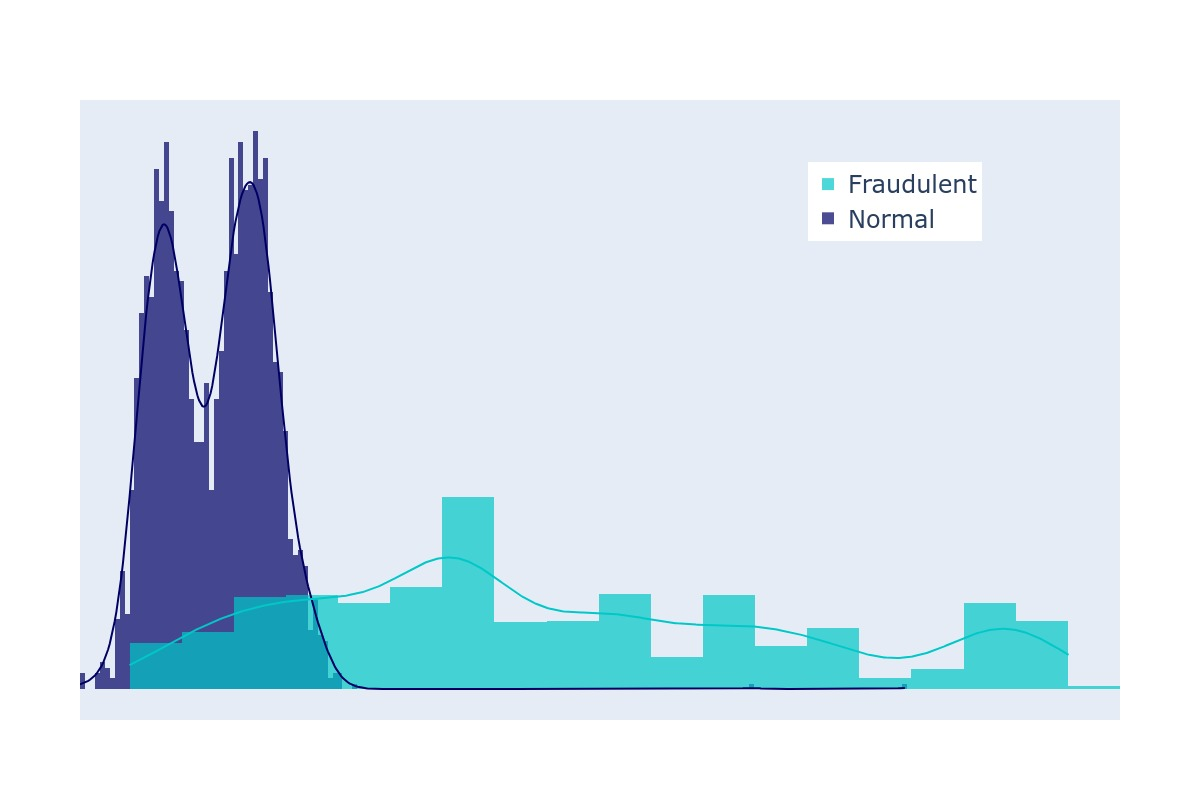
\includegraphics[width=\linewidth,trim=40 40 40 40,clip]{Figures/creditcard/PCA/SMOTE-data-run-0-0_DIST}
		\begin{tabular}{c|c|c|c}
			Fraud & Normal & Inter. & HDR  \\
			\hline
			2585  & 2585  & 534 & 20.66\(\%\) \\
		\end{tabular}
		\caption{Generated data by SMOTE. }
		\label{fig:SMOTE_hist}
	\end{subfigure}
	\\ 
	\begin{subfigure}[]{0.3\linewidth}	
		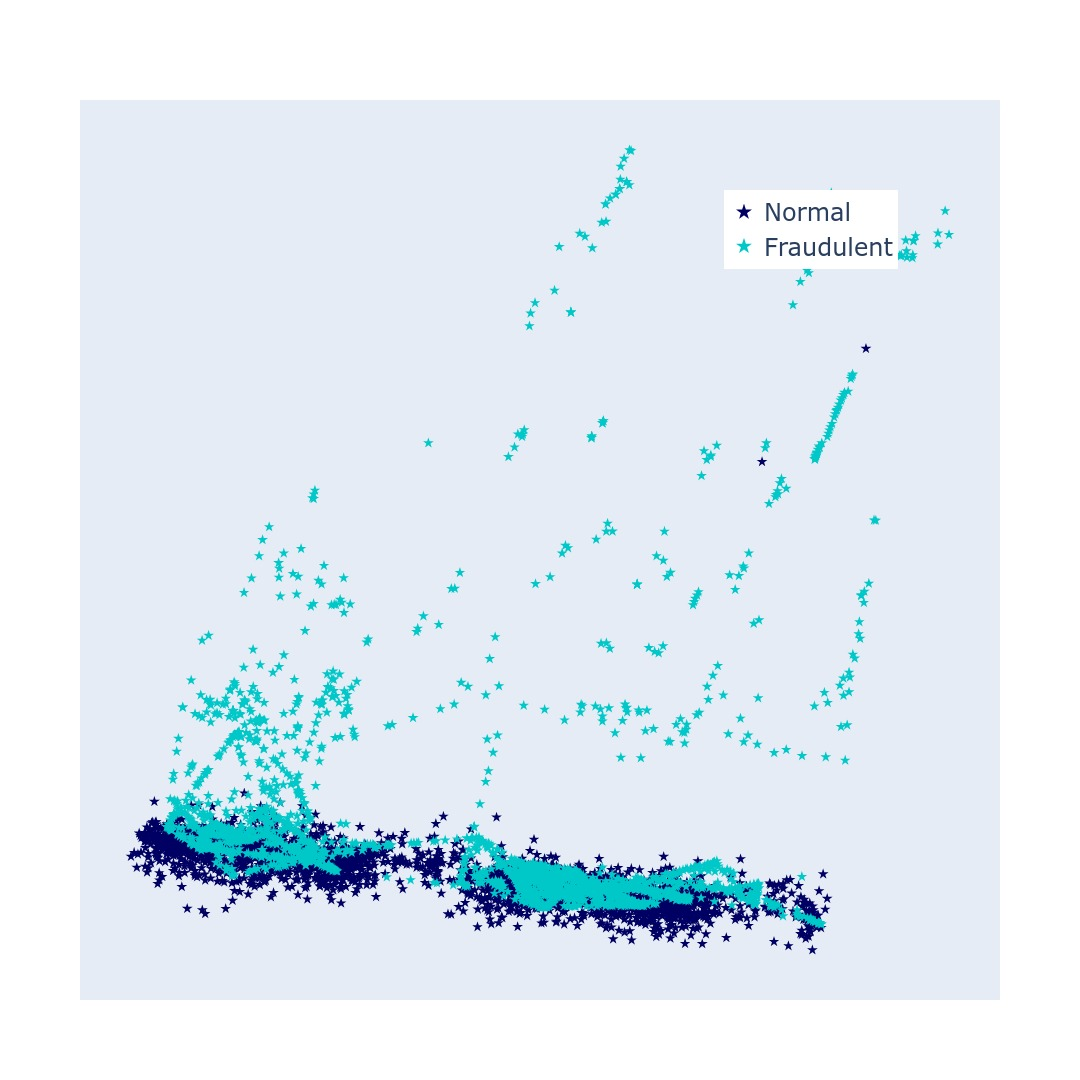
\includegraphics[width=\linewidth,trim=40 40 40 40,clip]{Figures/creditcard/PCA/ADASYN-data-run-0-0}
		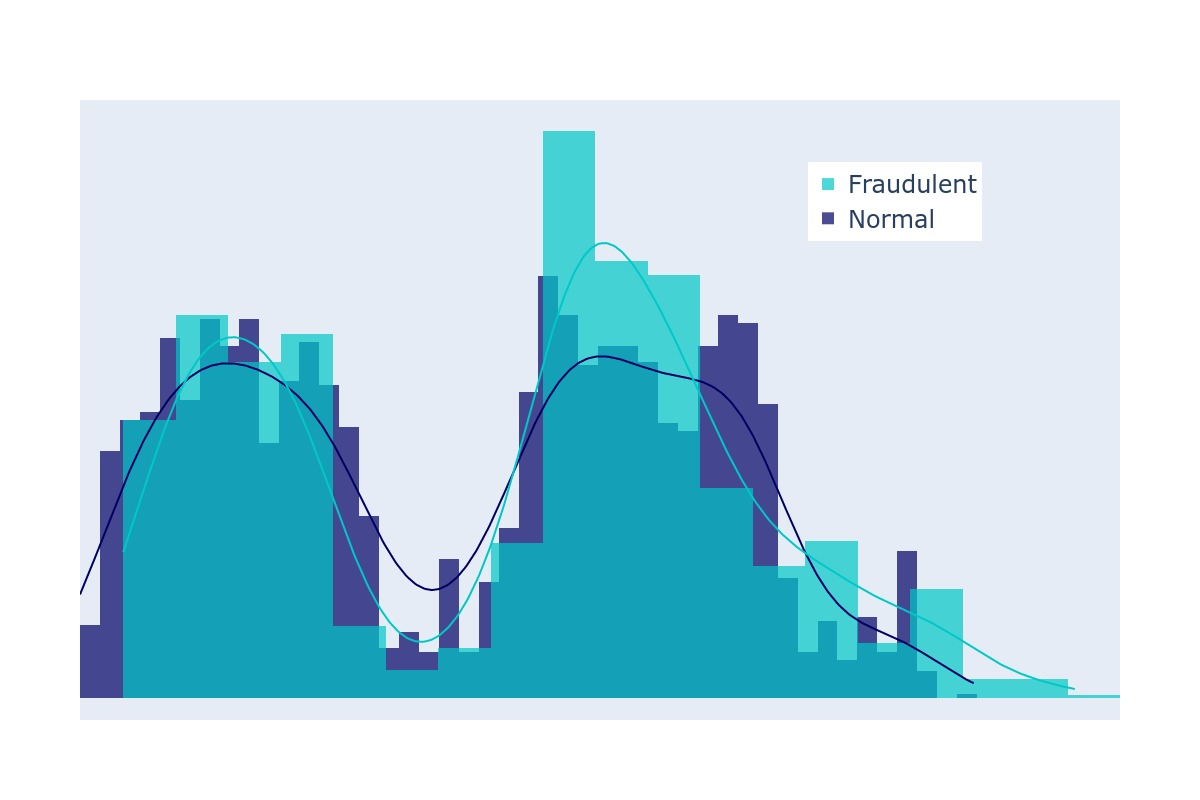
\includegraphics[width=\linewidth,trim=40 40 40 40,clip]{Figures/creditcard/PCA/ADASYN-data-run-0-0_DIST}
		\begin{tabular}{c|c|c|c}
			Fraud & Normal & Inter. & HDR  \\
			\hline
			2585  & 2585  & 2115 & 81.82\(\%\) \\
		\end{tabular}
		\caption{Generated data by ADASYN. }
		\label{fig:ADASYN_hist}
	\end{subfigure}
	\hspace{0.1em}%
	\begin{subfigure}[]{0.3\linewidth}	
		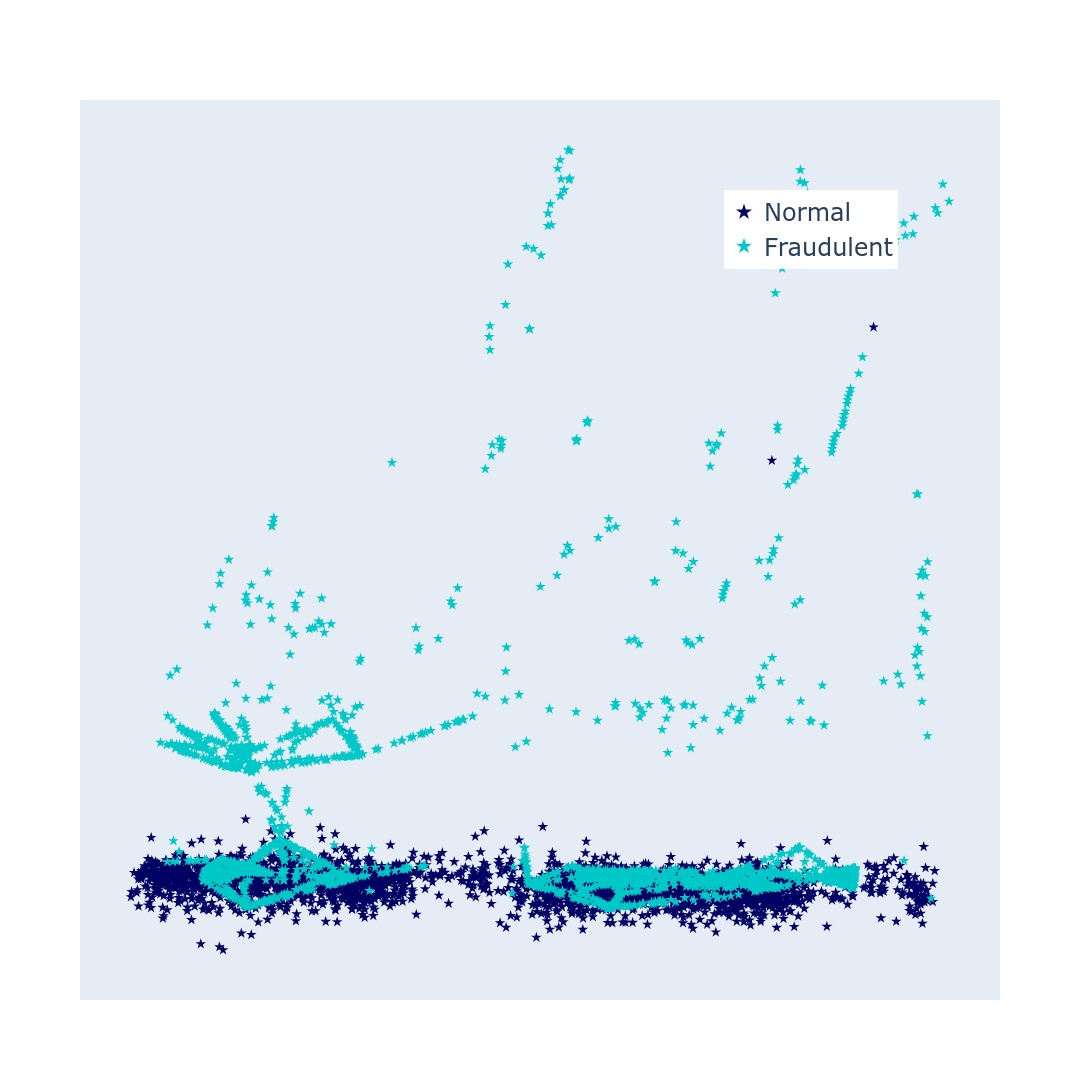
\includegraphics[width=\linewidth,trim=40 40 40 40,clip]{Figures/creditcard/PCA/BorderlineSMOTE-data-run-0-0}
		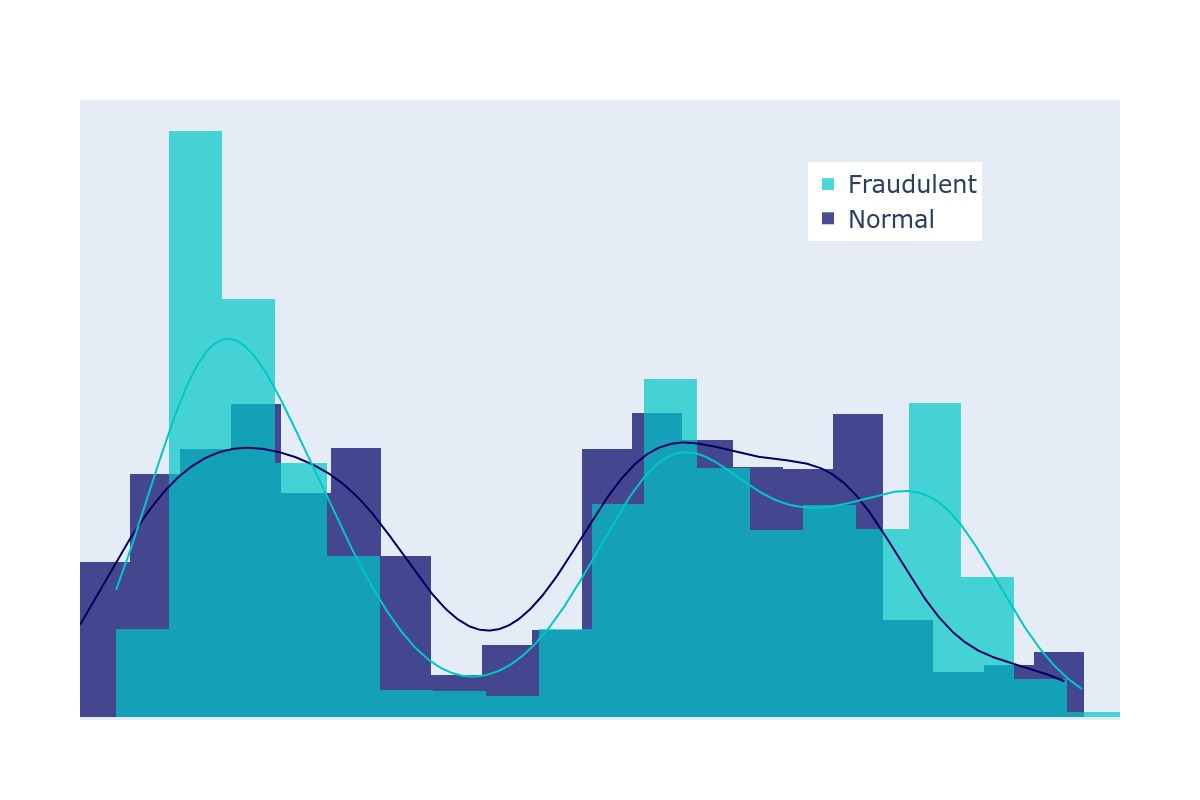
\includegraphics[width=\linewidth,trim=40 40 40 40,clip]{Figures/creditcard/PCA/BorderlineSMOTE-data-run-0-0_DIST}
		\begin{tabular}{c|c|c|c}
			Fraud & Normal & Inter. & HDR  \\
			\hline
			2585  & 2585  & 1964 & 75.98\(\%\) \\
		\end{tabular}
		\caption{Generated data by BorderlineSMOTE. }
		\label{fig:BorderlineSMOTE_hist}
	\end{subfigure}
	\hspace{0.1em}%
	\begin{subfigure}[]{0.3\linewidth}	
		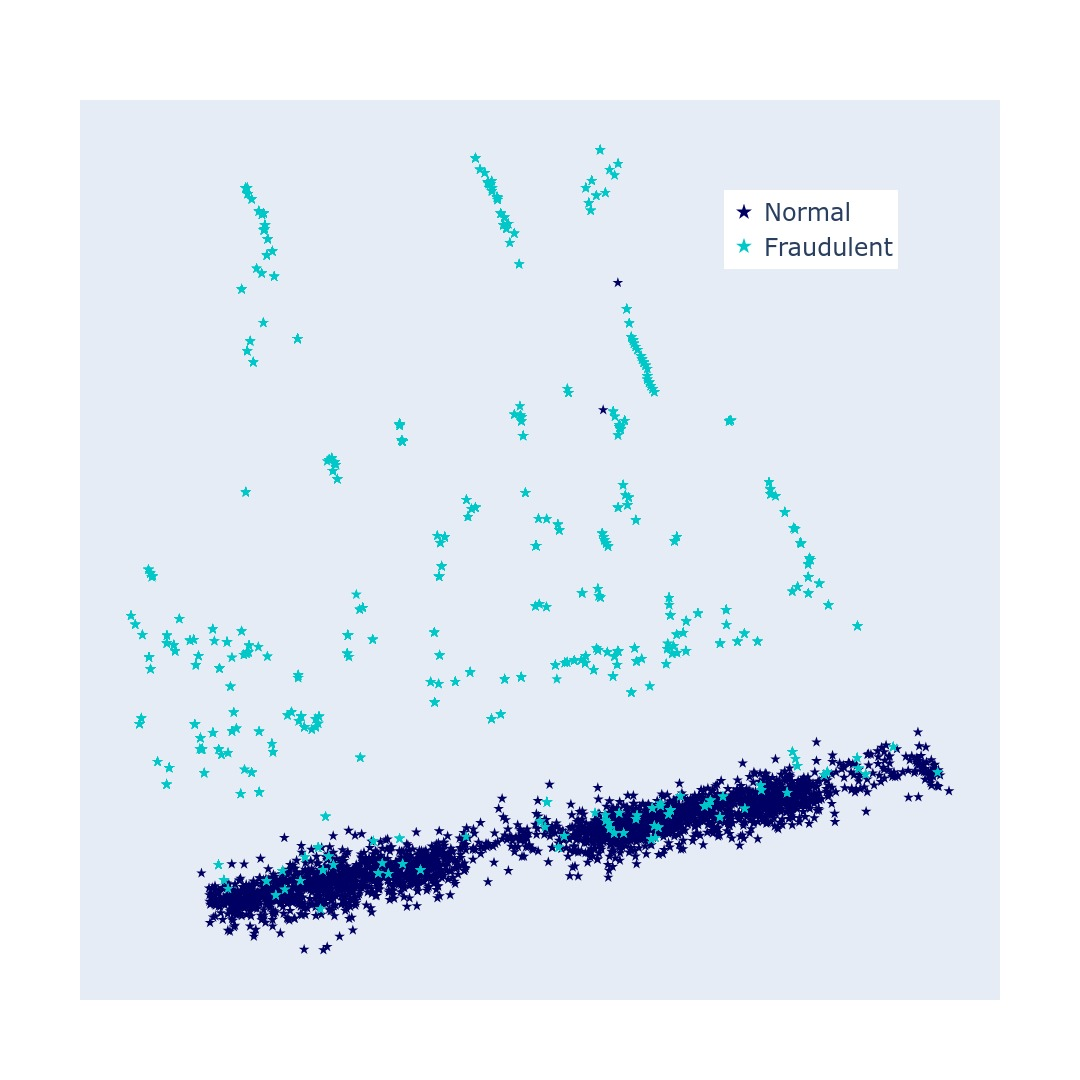
\includegraphics[width=\linewidth,trim=40 40 40 40,clip]{Figures/creditcard/PCA/Oversampling-data-run-0-0}
		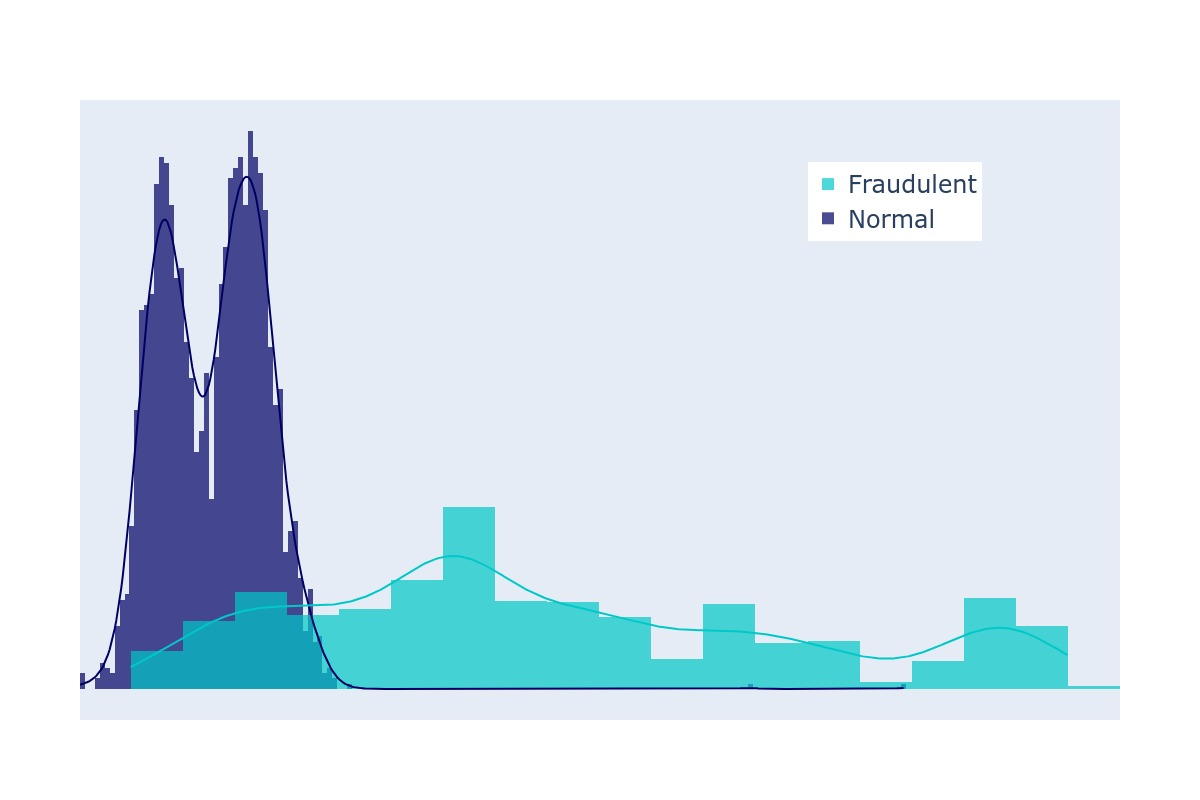
\includegraphics[width=\linewidth,trim=40 40 40 40,clip]{Figures/creditcard/PCA/Oversampling-data-run-0-0_DIST}
		\begin{tabular}{c|c|c|c}
			Fraud & Normal & Inter. & HDR  \\
			\hline
			2585  & 2585  & 544 & 21.4\(\%\) \\
		\end{tabular}
		\caption{Generated data by Oversampling. }
		\label{fig:Oversampling_hist}
	\end{subfigure}

	\caption{Generated training data projected onto 2-dimension space and their histograms in 1-Dimension space using Principle Component Analysis dimension reduction technique. The explanation tables illustrate the number of samples in each class (Fraudulent and Normal), 1-Dimension histogram intersection between 2 classes, and the hard-to-differentiate ratio ($HDR = \frac{Inter.}{Fraud}100\%$).}
	\label{fig:creditcard_plot}
	
\end{figure*}



\subsubsection{Dataset}
In this section, we experiment with our technique on Credit Card Fraud dataset \cite{goy_credit_2019}. The original dataset contains 492 fraud records out of 284,807 transactions; each record includes 30 features. During the experiments, we fix the size of fraud records as it becomes the minority class and randomly select a part of the remaining normal transactions to generate new datasets with different imbalance ratios. The classification model for the experiments under this dataset can be found in Table \ref{tab:model_setting}.

\subsubsection{Results and Discussions} 


\begin{table*}[ht]
	\centering
	\caption{Classification results of different data balancing techniques on Credit Card Fraud Dataset.}
	\label{tab:creditCardResult}%

		\begin{tabular}{rrcrcccccc}
			\toprule
			\multicolumn{10}{c}{\textbf{Credit Card Fraud}} \\
			&       &       &       &       &       &       &       &       &  \\
			\multicolumn{1}{c}{Majority:Minority} &       & Metric &       & \textbf{SIMPOR} & \textbf{SMOTE} & \textbf{Borderline} & \textbf{Over-} & \textbf{ADASYN} & \textbf{RawData} \\
			\multicolumn{1}{c}{(IR)} &       &       &       &       &       & \textbf{SMOTE} & \textbf{Sampling} &       &  \\
			\cmidrule{1-1}\cmidrule{3-3}\cmidrule{5-10}          &       & F1    &       & \textbf{0.943} & 0.903 & 0.865 & 0.939 & 0.821 & 0.879 \\
			\multicolumn{1}{c}{1470:490 } &       & AUC   &       & \textbf{0.968} & \textbf{0.968} & 0.967 & 0.967 & \textbf{0.968} & 0.966 \\
			\multicolumn{1}{c}{(3:1)} &       & Precision &       & \textbf{0.952} & 0.899 & 0.846 & 0.948 & 0.805 & 0.873 \\
			&       & Recall &       & \textbf{0.936} & 0.918 & 0.903 & 0.932 & 0.879 & 0.907 \\
			\cmidrule{1-1}\cmidrule{3-3}\cmidrule{5-10}          &       & F1    &       & \textbf{0.953} & 0.931 & 0.891 & 0.935 & 0.835 & 0.944 \\
			\multicolumn{1}{c}{3430:490 } &       & AUC   &       & \textbf{0.974} & \textbf{0.974} & 0.964 & \textbf{0.974} & \textbf{0.974} & 0.971 \\
			\multicolumn{1}{c}{(7:1)} &       & Precision &       & \textbf{0.975}  & 0.924 & 0.868 & 0.935 & 0.790  & \textbf{0.975} \\
			&       & Recall &       & \textbf{0.938} & \textbf{0.938} & 0.922 & 0.936 & 0.928 & 0.919 \\
			\cmidrule{1-1}\cmidrule{3-3}\cmidrule{5-10}          &       & F1    &       & \textbf{0.952} & 0.901 & 0.863 & 0.658 & 0.906 & 0.930 \\
			\multicolumn{1}{c}{4900:490 } &       & AUC   &       & \textbf{0.972} & 0.957 & 0.967 & 0.964 & 0.969 & 0.975 \\
			\multicolumn{1}{c}{(10:1)} &       & Precision &       & \textbf{0.979} & 0.891 & 0.855 & 0.662 & 0.885 & 0.931 \\
			&       & Recall &       & 0.929 & 0.925 & 0.918 & 0.845 & 0.933 & \textbf{0.936} \\
			\cmidrule{1-1}\cmidrule{3-3}\cmidrule{5-10}          &       & F1    &       & \textbf{0.952} & 0.909 & 0.885 & 0.917 & 0.883 & 0.944 \\
			\multicolumn{1}{c}{7350:490 } &       & AUC   &       & \textbf{0.968} & 0.963 & 0.955 & 0.963 & 0.965 & 0.960 \\
			\multicolumn{1}{c}{(15:1)} &       & Precision &       & 0.966 & 0.892 & 0.850  & 0.909 & 0.849 & \textbf{0.984} \\
			&       & Recall &       & \textbf{0.940} & 0.931 & 0.931 & 0.935 & 0.931 & 0.911 \\
			\bottomrule
		\end{tabular}%
	

\end{table*}%


Table \ref{tab:creditCardResult} shows the classification results on Credit Card Fraud dataset over different balancing techniques. \Methodname{} constantly overperforms other techniques over all the settings and achieves the highest F1 and AUC score. While SIMPOR, SMOTE improve classification performance in most of the settings, ADASYN, BorderlineSMOTE fail to create good synthetic samples and reduce the classification performance.       

To better understand how the techniques perform, we visualize the generated data by projecting them onto lower dimensions (i.e., one and two dimensions) space using the Principle Component Analysis technique (PCA) \cite{pca}. Data's 2-Dimension (2D) plots and 1-Dimension histograms are presented in Figure \ref{fig:creditcard_plot}. A hard-to-differentiate ratio (HDR) is defined as the ratio of intersection between 2 classes in the 1D histogram to the total Fraudulent samples ($HDR = \frac{No.\: Intersection \: samples}{No. \: Fraud \: samples} $). This ratio is expected to be as small as 0\% if the two classes are well separated; in contrast, 100\% indicates that the two classes are unable to be distinguished. Other than HDR, the bottom tables in Figure \ref{fig:creditcard_plot} also show the absolute numbers of Fraudulent, Normal, and Intersection samples for each technique. From the plots, we can observe how the data distribute in 2D space and quantify hard-to-differentiate samples in the histograms. 

While some techniques help to reduce the hard-to-differentiate ratios, others increase this ratio and worsen the data distribution. For example, in the 1D histogram of the ADASYN technique (Figure \ref{fig:ADASYN_hist}), there are 2115 samples in the histogram intersection between 2 classes; they account for 81.82\% of the total 2585 Fraudulent samples, which is worse than HDR of the Rawdata case (69.75\%). In addition, the 2-Dimension plot illustrates that many synthetic samples (Fraudulent class) cross the majority (Normal class). Similarly, Figure \ref{fig:BorderlineSMOTE_hist} shows that BorderlineSMOTE also poorly generates synthetic minority data in this setting (CreditCard Fraudulent dataset with IR of 7:1) with an HDR of 75.98\%. Among all techniques, \Methodname{} achieves the best HDR of 11.14\% and the synthetic data are far away from the majority class, which helps to improve the classification results as shown in Table \ref{tab:creditCardResult}.

